%-------------------------------------------------------------------------------
\subsection{Granting Liveness}
%-------------------------------------------------------------------------------
\sys operates under the premise that clients experience progress indepentently - there exists no shared notion of system progress. Byzantine clients, may bring execution, validation or writeback to a halt for their own transactions: they may stall during all phases, or equivocate during validation logging, causing replicas to diverge on decision values (Commit/Abort) and thus prohibiting the generation of shard-certificates. When all transactions are commutative this phenomenon requires no action: Any client \textit{chooses} whether to adhere to the protocol and experience progress, or not. However, when transactions depend on each other, either explicitly by claiming dependencies on uncommitted write), or implicitly through read-write conflicts, liveness is no longer independent. For instance, a dependency that does not progress may cause the dependent to block indefinetely, while an uncommited, but insufficiently replicated, write might cause consecutive read transactions to abort.
In order to allow clients to safely intertwine their fate with concurrent transactions, \sys must provide clients the tools reclaim their own liveness. We define Liv: 
\begin{theorem}[Liv] 
Every transaction that an honest client is \textit{interested} in eventually completes.
\end{theorem}

Intuitively, honest clients enjoy this progress property granted that they can reliably obtain shard-certificates as any client can conduct the writeback phase. To achieve this, we must relax the requirement that replicas may never alter their decision, while preserving Theorem Saf.

A naive solution that allows any client to drive another clients protocol is problematic, since \textit{interested} clients could concurrently make inconsistent decisions, thus inhibiting progress. Likewise, coordinator election across client is undesirable as there may exist an unbounded number of electable byzantine clients that may not constructively aid in reconciliation. In \sys we circumvents this by letting concurrent clients replay non critical sections of the protcol, while delegating critical responsibility to the bounded replica set. Concretely, we design a mechanism to endorse a dedicated \textit{Fallback} replica responsible for reconciling diverged replica decisions. Since the number of faulty replicas is bounded, at most $f+1$ leader elections are necessary to make progress when the network is synchronous. \sys challenge is to guarantee a live round-robin election while keeping clients responsible for their own progress. We remark, that in an asynchronous network, deterministic leader election might not be possible  \cite{fischer1985impossibility}.  \fs{no non-randomized protocol can reach agreement in an async setting. (randomized exceptions: BenOr, Honeybadger, BEAT)}.

On a high level, the recovery mechanism operates as follows: \textit{Interested} clients attempt to run the validation protocol themselves. If a client suspects decision divergence, it issues a \textit{Fallback invocation} request, electing a \textit{Fallback} replica that reconcile decisions. Such recovery protocol is reminiscent of \textit{view-changes} in traditional BFT SMR protocols, but differs in two core aspects: a) While control changes between fallback replicas (leaders), the protocol is still client driven and linear in complexity, and b) The fallback mechanism impacts only the ongoing transaction. Independent concurrent transactions are unaffected. Figure \ref{fig:FigureFBnom} shows an example scenario requiring reconciliation, and gives on overview of the  Fallback protocol message pattern.

\begin{figure}
\begin{center}
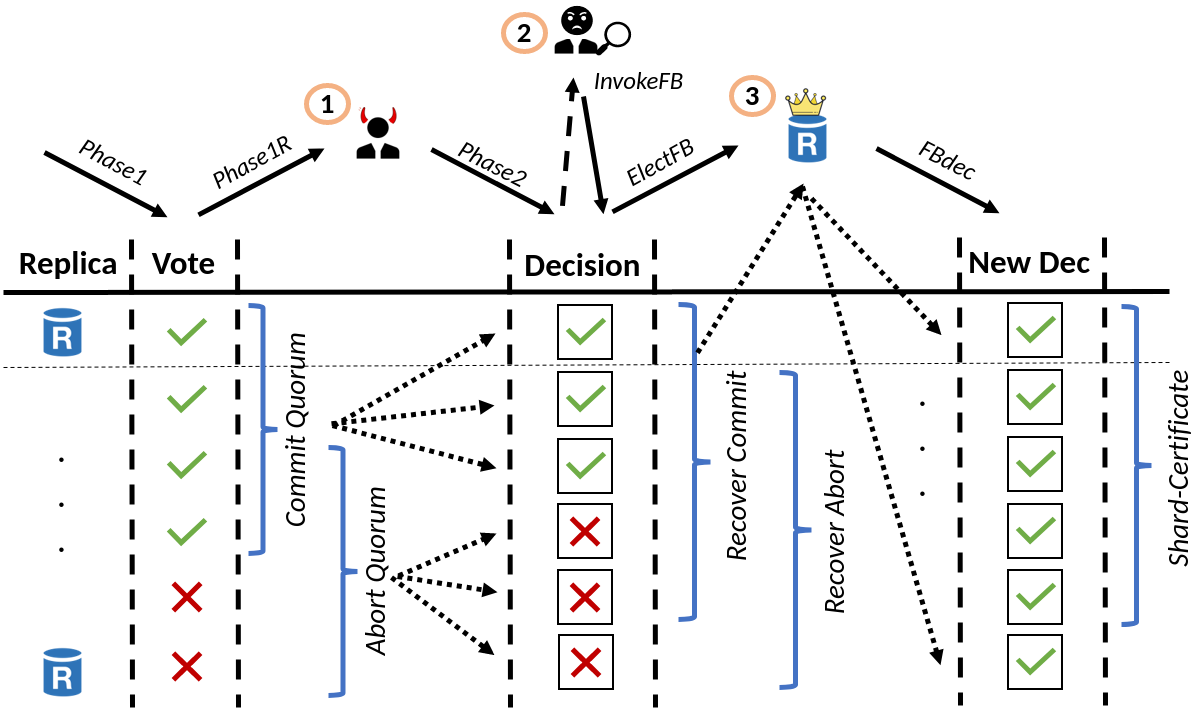
\includegraphics[width= 0.5\textwidth]{./figures/FBNom.png}
\end{center}
\caption{Fallback Scenario. 1. A byzantine client equivocates decisions. 2. An interested client invokes a Fallback Replica (FB) election. 3. An honest FB reconciles a single decision.}
\label{fig:FigureFBnom}
\end{figure}


Below, we detail the protocol by following a transactions life cycle. To start the protocol we assume an \textit{interested} client is in possession of the respective transactions $Prepare$ request, signed by the orignial issuer. This information may be obtained during the validation of the clients own transaction, either as full dependency or conflict. 
%%%%%%%%%%%%%%%%%%%%%%%%%%%%%%%%%%%% WRITEBACK HAS ALREADY HAPPENED


%%Cut the protocol re-iterations?

\fbox{\begin{minipage}{23em}
\textbf{(1: C $\rightarrow$ R)}: Client issues Prepare request and inquires current protocol state.
\end{minipage}}\\
An interested client broadcast a message $Backup-Phase1 \coloneqq (TX.Phase1, CID)$ to all replicas in \textit{InvolvedShards} of the transaction. \\
\fbox{\begin{minipage}{23em}
\textbf{(2: R $\rightarrow$ C)}: Replica marks Client as interested and returns its state.
\end{minipage}}\\
Replicas execute an un-seen $Phase1$ (see Validation, step 2), and reply with its vote. Otherwise, a replica replies with its current decision value and the corresponding view ($Phase2R$), or, if not existant, with its origninal vote ($Phase1R$), and lastly, its current view.\\
\underline{Finalized decisions:} If a replica has already received a Writeback message for a transaction it ignores all Fallback related client requests and simply returns the decision and corresponding certificate. An intersted client can return to the Writeback phase immediately and forward the response.\\
\fbox{\begin{minipage}{23em}
\textbf{(3a: C $\rightarrow$ R)}: A client receives the necessary information to proceed to Writeback.
\end{minipage}}\\
A client either a) receives a Fast-Path threshold of $Phase1R$ messages, or b) receives sufficiently many matching (in decision and view) $Phase2R$ messages to assemble a shard-certificate. \\
\fbox{\begin{minipage}{23em}
\textbf{(3b: C $\rightarrow$ R)}: A client needs to go Slow-Path or observes inconsistency and requires assistance for resolution.
\end{minipage}}\\
If a client receives insufficient $Phase2R$ replies to return, the client itself broadcasts $Phase2$ messages using the received $Phase1R$ or $Phase2R$ responses as proof in order to log a decision. If instead, a client receives inconsistent $Phase2R$ replies (either decision or view), it invokes a fallback election, broadcasting a message $InvokeFB \coloneqq (TxID, CID, \{view\}_R$ that includes a Quorum of replicas' current views.
Inconsistent replies from the same view $v$ additionally constitute a Proof of Misbehavior (PoM) for the issuing client or replica. \\
\fbox{\begin{minipage}{23em}
\textbf{(4a: R $\rightarrow$ C)}:  Replicas receive $Phase2$ messages and replies with decision
\end{minipage}}\\
A replica buffers requests until the orginial client timer expires, and, upon expiration, adopts the decision if it has stored none. It returns a corresponding $Phase2R$ message. \\
\fbox{\begin{minipage}{21em}
\textbf{(4b: R $\rightarrow$ R(FB))}: Replicas receives Fallback invocation and starts election
\end{minipage}}\\
If a replica receives an $InvokeFB$ message and the original client has timed-out it attempts to elect a new \textit{Fallback replica}. To do so, it follows the \textbf{View Change Rules} and adopts new view $current.view = v+1$ if $v \geq current.view$. 
Replicas send an $ElectFB \coloneqq (TxID, decision, current.view)_R$ to replica $current.view + TxID \% n$. \\
\underline{\textbf{View Change Rules:}} \one Replicas only adopt a view $v+1$ if the view set includes $3f+1$ votes from view $v$. \textit{Vote subsumtion:} A view $v$ may count as a vote for all $v' \leq v$. \two Replicas that lag behind, may safely skip ahead to the maximum view $v$ present $f+1$ times, since, by induction, $\geq 3f+1$ replicas must have claimed to be in a view $\geq v-1$. Thus, any possible divergence can be reconciled in a single step, as there must exist a view $v' \geq max(honest.views) -1 $ for which at least $f+1$ honest votes exist in any Quorum of $4f+1$ votes.\\
\underline{Additional subtlelties:} Replicas enforce exponential time-outs for new elections. In absence of honest interested clients, byzantine clients may invoke fallback elections at a subset of replicas, thus inhibiting true election and skipping select replicas' terms. To avoid artificially increased timeouts and non-skipping candidates, replicas may forward the $ElectFB$ message to all other replicas. Replicas that receive $f+1$ forwarded messages, adopt larger views, and forward the $ElectFB$ message themselves, thus ensuring election for each view.
\footnote{This optimization is not necessary for "theoretical" liveness. To avoid unecessary all-to-all communication, it may only be enforced for views $v > T$, where T is a system hyperparameter }\\
\fbox{\begin{minipage}{21em}
\textbf{(5: R(FB) $\rightarrow$ R)}:  Fallback aggregates and echos election messages.
\end{minipage}}
The Fallback replica considers itself elected upon receiving a Quorum of $4f+1$ ElectFB messages. It then uses this set of messages to reconcile a decision. It broadcasts a message $FBdec \coloneqq \langle RID, dec, view, \{ElectFB_r\} \rangle_R$, including proof for the new decision. \\
\textbf{Decision Reconciliation Rule:} \textit{$dec_{new}$ $=$ maj(\{Elect.decision\})}. If a logged decision exists (implies that a shard-decision might exist), any Quorum of $4f+1$ Elect messages is guaranteed to contain $2f+1$ matching decisions (a majority). Otherwise, an arbitrary decision qualifies since at least one honest replica must have agreed to it.\\
\underline{Additional subtlelties:} The attentive reader may notice that Elect messages do not include a corresponding view. Decisions need not match in views: By the Decision Reconciliation Rule, if there ever existed a logged decision $d$ with matching views, then all future $dec_{new} = d$.\\
\fbox{\begin{minipage}{21em}
\textbf{(6: R $\rightarrow$ C)}:  Replicas echo decision to interested clients
\end{minipage}}
Replicas receive a $FBdec$ message, adopt $decision = (FBdec.dec, FBdec.view)$ and $current.view = FBdec.view$ if $FBdec.view \geq current.view$, and forward the respective decision to all interested clients. Replicas that time out waiting for a $FBdec$ message proactively forward their current view to all interested clients. \\
\fbox{\begin{minipage}{21em}
\textbf{(7: C}: A client starts Writeback phase or restarts Fallback invocation
\end{minipage}}
An interested client returns to the Writeback phase upon receiving sufficiently matching decisions. If it times out, or receives inconsistent decisions it inquires a new set of current views and re-starts Fallback starts a new broadcast $InvokeFB \coloneqq (TxID, CID, \{view\}_R$.\\
\underline{Additional subtlelties:} An honest client \textit{expects} to receive $4f+1$ matching decisions and will continue to wait for decisions from the same view up to a timeout. Eventually a logged decision must exist and time-outs grow enough to guarantee a client will receive a shard-certificate. \fs{In section X (optimization) we discuss a practical optimization: Async extra phase.}\\
%%%%%%%
Given synchrony, any honest client that follows the Fallback protocol experiences \textit{Liv}. This follows straightforward from the eventual existance of an honest Fallback replica (at most $f+1$ elections) that reconciles all honest replicas. For any transaction, an interested honest client will eventually receive a shard-decision, and hence the transaction will complete.

We point out that steps 1, 2a, 3 and 4a simply correspond to the normal validation protocol. In order to avoid (multiple) \textit{interested} clients interfering too soon and causing unecessary divergence, we grant the original client an initial window of immunity.\footnote{Note, that it is irrelevant which client issues the $Phase1$ message. Therefore, we enforce the timeout window only for explicit logging ($Phase2$).} The orignial client is an interested client by default - an honest client that loses autonomy will, if necessary, elect a \textit{Fallback} itself. 

When depending on slow or byzantine transactions, clients may have to incur addtional latency in order to maintain liveness. On the flipside, when a clients fate is independent from other transactions, it is unaffected by concurrent slowdowns. 
